\section{Evaluation Methodology}
This section reports the observed performance of the running Patchwork-Service implementation under nine 100-request concurrency tests. The experiments examine worker-count scaling and changes to container-pool configuration. They do not include a measured per-submission on-demand-container baseline; consequently, the results characterize the tested warm-pool deployment and its operational limits rather than quantify a causal latency reduction relative to cold container creation.

\subsection{Experimental Setup}
\textbf{Execution host and load generator.} The service and load generator ran on separate machines. Table~\ref{tab:environment} summarizes the hardware and software details available from the benchmark record. Exact server CPU model, Docker version, storage details, and the Redis/RQ versions were not recorded in that report and are therefore not inferred here.

\begin{table*}[t]
\centering
\caption{Hardware and Software Environment Reported for the Benchmark}
\label{tab:environment}
\renewcommand{\arraystretch}{1.12}
\setlength{\tabcolsep}{5pt}
\begin{tabular}{p{0.15\textwidth}p{0.37\textwidth}p{0.37\textwidth}}
\toprule
\textbf{Parameter} & \textbf{Service host} & \textbf{Load generator} \\
\midrule
Processor & Intel Core i5, 12th generation (exact model not recorded in benchmark report) & Intel Core Duo (exact model not recorded) \\
Memory & 16 GB & 12 GB \\
Operating system & Linux Mint, terminal-only mode & Linux Mint XFCE \\
API / runtime & FastAPI 0.139.0; Python 3.12.3 & Node.js 22.23.3; k6 2.3.0 \\
Queue and execution & Redis / RQ; Docker-managed execution containers & k6-based concurrent request generation \\
\bottomrule
\end{tabular}
\end{table*}

\textbf{Workload and procedure.} Each of the nine tests issued 100 concurrent requests and used a 180-s grace period. The API request and callback workflow was kept generally consistent across the sequence. The first five tests varied the RQ worker count over $\{1,2,4,8,16\}$ while retaining a maximum pool size of 10 containers. Tests~6--9 used a configured maximum pool size of 20 and compared worker counts of 16, 10, 8, and 6, respectively. The supplied benchmark record describes one run for each configuration; repeated trials and confidence intervals were not available.

\begin{table}[t]
\centering
\caption{Container-Pool Settings by Test Group}
\label{tab:pool-settings}
\renewcommand{\arraystretch}{1.12}
\setlength{\tabcolsep}{3.4pt}
\begin{tabular}{p{0.43\columnwidth}cc}
\toprule
\textbf{Setting} & \textbf{Tests 1--5} & \textbf{Tests 6--9} \\
\midrule
Initial warm containers & 5 & 5 \\
Maximum pool size & 10 & 20 \\
Provisioning concurrency & 2 & 5 \\
Configured acquisition timeout & 10 s & 30 s \\
Framework target buffer & 5 & 12 \\
Redis pool target & 5 & 5 \\
\bottomrule
\end{tabular}
\end{table}

The settings in Table~\ref{tab:pool-settings} are the configured values reported for each group; they are not proof that every live process had loaded the corresponding values. In particular, Test~6 recorded container-acquisition failures after approximately 10.2--10.4~s despite the configured 30-s timeout. The benchmark notes that workers had not been restarted after the configuration change, so stale worker configuration is a plausible explanation, but the available evidence does not establish it as the only cause.

\subsection{Metrics}
The dashboard-reported throughput is expressed in requests per second. We also report total test elapsed time and end-to-end completion latency, measured from request submission until the callback response was received. Mean, median, and 95th-percentile (P95) latency are included where recorded. End-to-end latency includes queueing, container acquisition, workspace preparation, execution, cleanup, and callback delivery; it is not equivalent to code execution time. For Test~6, the detailed export additionally reported queue delay and worker timing. Failure observations are reported conservatively: the phrase ``no failure banner shown'' is not interpreted as proof of zero failed executions, and missing dashboard failure counts are not treated as zero.

\subsection{Results}
Table~\ref{tab:all-results} summarizes all nine tests in the order in which the experiments were reported. Pool maxima refer to configured maximum container counts. The failure column records only what was visible in the supplied dashboard or detailed export.

\begin{table*}[t]
\centering
\caption{Results of the Nine 100-Request Concurrency Tests}
\label{tab:all-results}
\renewcommand{\arraystretch}{1.08}
\setlength{\tabcolsep}{4.2pt}
\small
\begin{tabular}{rrrrrrrr>{\raggedright\arraybackslash}p{2.15cm}}
\toprule
\textbf{Test} & \textbf{Workers} & \textbf{Pool max.} & \textbf{Elapsed (s)} & \textbf{Mean (s)} & \textbf{Median (s)} & \textbf{P95 (s)} & \textbf{Throughput (req/s)} & \textbf{Failure evidence} \\
\midrule
1 & 1  & 10 & 152.8 & 80.05 & 79.84 & 145.26 & 0.655 & No banner shown \\
2 & 2  & 10 & 90.4  & 44.26 & 43.54 & 85.86  & 1.108 & No banner shown \\
3 & 4  & 10 & 60.9  & 29.17 & 27.84 & 57.30  & 1.647 & No banner shown \\
4 & 8  & 10 & 43.3  & 20.68 & 19.41 & 41.83  & 2.314 & No banner shown \\
5 & 16 & 10 & 37.9  & 18.35 & 16.30 & 35.66  & 2.645 & 6 failures \\
6 & 16 & 20 & 55.7  & 36.03 & 33.28 & 54.25  & 1.801 & 6 failures \\
7 & 10 & 20 & 51.2  & 31.14 & 28.49 & 50.40  & 1.957 & Count unavailable \\
8 & 8  & 20 & 44.6  & 22.17 & 20.82 & 41.75  & 2.247 & Count unavailable \\
9 & 6  & 20 & 49.2  & 23.39 & 21.36 & 47.81  & 2.039 & Count unavailable \\
\bottomrule
\end{tabular}
\end{table*}

\begin{figure*}[t]
\centering
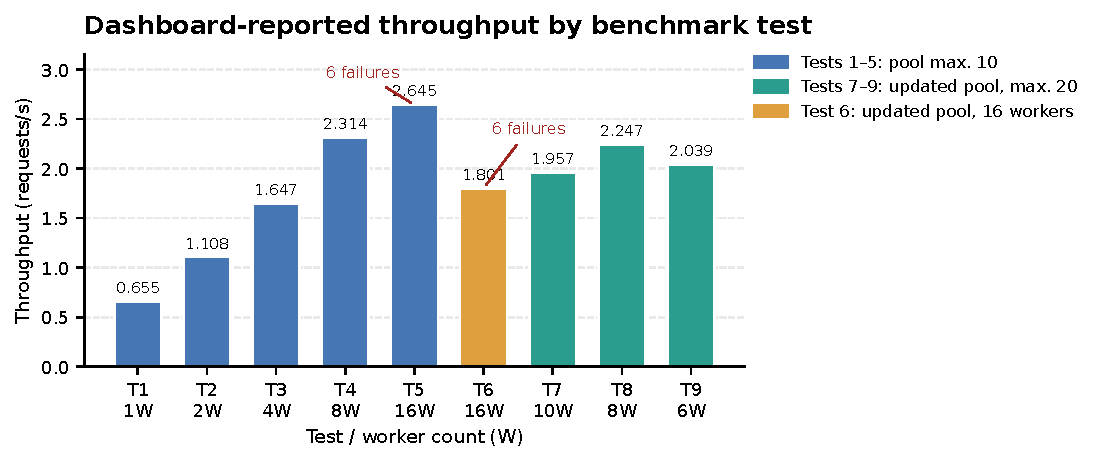
\includegraphics[width=0.92\textwidth]{figures/throughput.pdf}
\caption{Dashboard-reported throughput across the nine tests. Tests~1--5 used a maximum pool size of 10; Tests~6--9 used a configured maximum of 20 with other pool settings changed. The two tests with six reported failures are annotated.}
\label{fig:throughput}
\end{figure*}

\begin{figure*}[t]
\centering
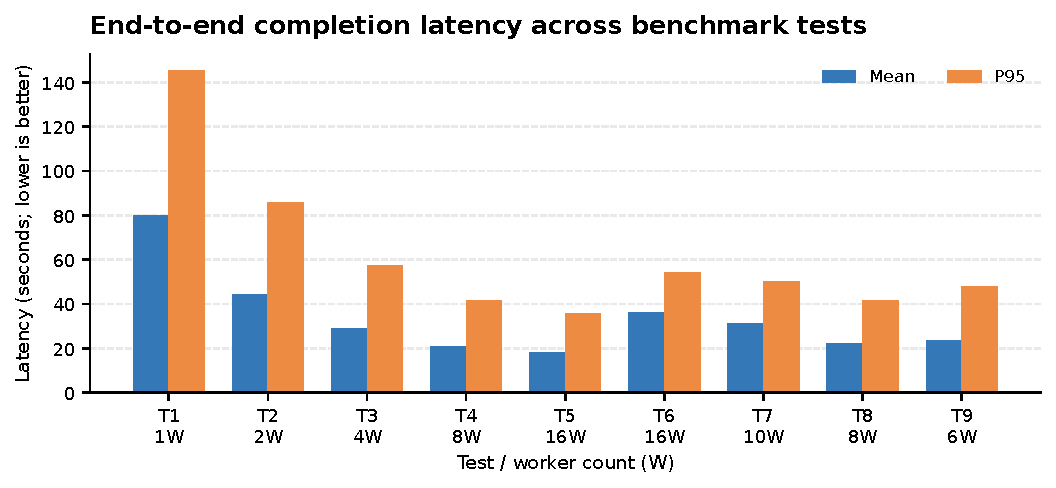
\includegraphics[width=0.92\textwidth]{figures/latency.pdf}
\caption{Mean and P95 end-to-end completion latency for each test. Both measures include asynchronous queueing and callback delivery; lower values indicate shorter observed completion times.}
\label{fig:latency}
\end{figure*}

\subsection{Discussion}
\textbf{Worker-count scaling with the original pool.} As shown in Fig.~\ref{fig:throughput}, the first four tests increased dashboard throughput from 0.655~requests/s with one worker to 2.314~requests/s with eight workers. Over the same comparison, mean end-to-end latency decreased from 80.05~s to 20.68~s, a reduction of approximately 74.2\%. This indicates that additional workers substantially improved aggregate processing capacity over the lower worker counts in this workload. Increasing to 16 workers produced the highest observed raw throughput, 2.645~requests/s, and the lowest observed mean latency in the original-pool group (18.35~s), but six container-acquisition failures were reported. Thus, the Test~5 result should not be interpreted as the best reliable operating point solely on the basis of throughput.

\textbf{Tests with the updated pool configuration.} Among Tests~6--9, the eight-worker configuration (Test~8) had the highest dashboard throughput (2.247~requests/s) and the lowest mean and P95 latency (22.17~s and 41.75~s, respectively). It outperformed the ten-worker run (Test~7: 1.957~requests/s, 31.14-s mean, 50.40-s P95) and the six-worker run (Test~9: 2.039~requests/s, 23.39-s mean, 47.81-s P95) on these dashboard-level measures. However, the separate failure count was not visible for Tests~7--9; the evidence therefore supports describing eight workers as the best observed performance balance in this subset, not as a validated failure-free configuration.

\textbf{Container acquisition and queueing.} Tests~5 and~6 each reported six failures associated with inability to acquire a warm container. The detailed Test~6 export recorded approximately 28.612~s of mean queue delay and 36.034~s of mean end-to-end completion time, so queue delay represented about 79.4\% of the latter. The six failed submissions, however, had queue delays of only approximately 9--14~ms and failed after about 10.2--10.4~s with a container-acquisition error. This distinction indicates that queue waiting for successful jobs and container-acquisition failure were separate observed failure/performance paths in Test~6. The export also reported mean execution time of about 4.51~s, workspace creation of 0.64~s, cleanup of 0.68~s, and total worker time of about 6.86~s; these fields represent different timing intervals and should not be summed to reconstruct end-to-end latency.

\textbf{Interpretation and threats to validity.} The diminishing and inconsistent benefit at higher worker counts is consistent with contention for host resources and with a mismatch between worker concurrency and warm-container supply. Nevertheless, CPU utilization, per-core saturation, memory pressure, swap activity, disk I/O, and time-series pool occupancy were not collected. CPU saturation is therefore a plausible hypothesis rather than a directly measured cause. The experiment also changed multiple pool parameters between test groups, did not confirm that every worker loaded the updated timeout, used one reported run per configuration, and did not expose failure counts for three later tests. Finally, the available data do not include an on-demand-container baseline, per-configuration pool-hit rates, or correctness results (the dashboard reported correct results as unavailable). These limitations preclude a quantitative claim that warm pooling reduced latency relative to on-demand creation.

\subsection{Provisional Configuration}
For the next controlled experiment, the observed results support using eight workers as a provisional starting point with five initial warm containers, a configured pool maximum of 20, provisioning concurrency of five, a 30-s acquisition timeout, framework target buffer of 12, and Redis pool target of five. Before drawing a stable-performance conclusion, all worker processes should be restarted and checked for the active timeout, the number of pool daemons should be verified, and CPU, memory, swap, disk I/O, and idle/busy/provisioning container counts should be captured during the run. The eight-worker test should be repeated at least three times, and successful executions, infrastructure failures, missing callbacks, and correctness outcomes should be reported separately. A direct comparison against a matched on-demand baseline is required to quantify the latency benefit attributable to container reuse.
